\documentclass{beamer}
\usepackage{minted}
\usepackage{hyperref}
\usepackage{caption}
\captionsetup[figure]{labelformat=empty,font=scriptsize}
\hypersetup{
    colorlinks=true,      
    urlcolor=red,
    pdfpagemode=FullScreen,
}
\usetheme{CambridgeUS}
\title{Near-real time processing using Spark}
\subtitle{RDDs, DataFrame/DataSet, Spark Streaming, and Structured Streaming}
\author[Vladimir Siv\v{c}evi\'{c}]{Vladimir Siv\v{c}evi\'{c}}
\institute[Data Engineer]{Senior Data Engineer\\[2ex]www.vladsiv.com}
\date{\today}

\setbeamertemplate{section in toc}[ball unnumbered]
\setbeamertemplate{subsection in toc}[ball unnumbered]

\usepackage{minted}

\begin{document}

\frame{\titlepage}

\begin{frame}{Table of Contents}
	\tableofcontents[pausesections]
\end{frame}

\section{RDDs}
\begin{frame}[fragile]{RDD}
	RDD - Resilient Distributed Dataset
	\begin{itemize}
		\item<2-> \textbf{Resilient}
		\begin{itemize}
			\item<3-> \textbf{Immutable} - Rebuild lost data
			\item<4-> \textbf{Fault Tolerant} - Recover data using Lineage
		\end{itemize}
		\item<5-> \textbf{Distributed} - Across nodes, operated on in parallel
		\item<6-> Two ways to create them
		\begin{itemize}
			\item<7-> {
				\textit{Parallelized Collections}
				\scriptsize
				\begin{minted}{python}
data = [1, 2, 3, 4, 5]
distData = sc.parallelize(data)
				\end{minted}
			}
			\item<8-> 
			{
				\textit{External Datasets} - Any Hadoop supported storage - HDFS, S3, HBase...
				\scriptsize
				\begin{minted}{python}
distFile = sc.textFile("data.txt")
				\end{minted}
			}
		\end{itemize}
		\item<9-> \textbf{Partitions} - How is data distributed, determined by number of cores
				\scriptsize
				\begin{minted}{python}
sc.parallelize(data, 10)
				\end{minted}
		\item<10-> Generally unstructured data
	\end{itemize}
\end{frame}

\begin{frame}{RDD}
	\begin{center}
		\begin{figure}
			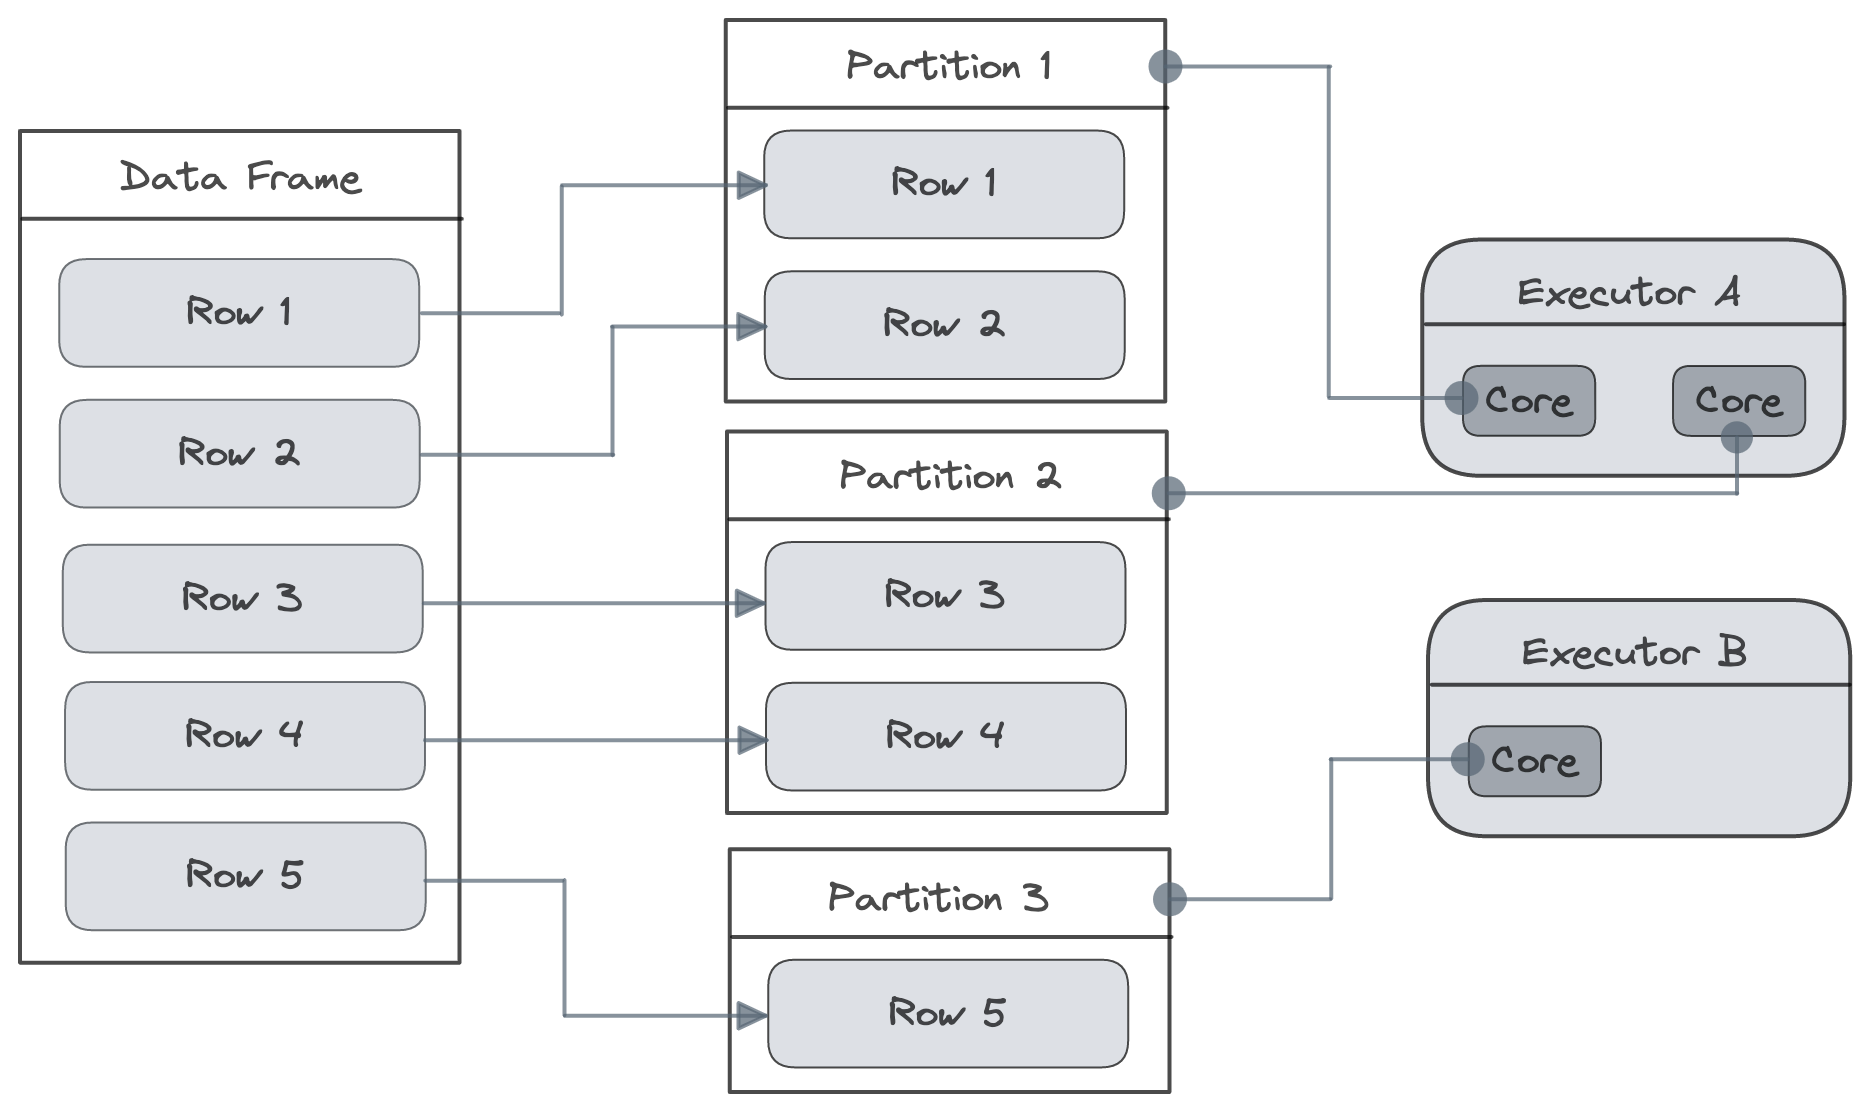
\includegraphics[height=6cm]{spark-data-partitions.png}	
			\caption{Image 1 - Partitions}
		\end{figure}
	\end{center}
\end{frame}

\begin{frame}[t]{RDD}
	RDDs support two type of operations:
	\begin{itemize}
		\item<1-> \textbf{Transformations} - create a new dataset from an existing one i.e. creates a completely new RDD
		\begin{itemize}
			\item<2-> \mintinline{java}{map()} - applies function to each element of a dataset and returns new RDD
			\item<3-> All transformations are lazy - think DAG
		\end{itemize}
		\item<3-> \textbf{Actions} - return a value to the driver program after running a computation on the dataset
		\begin{itemize}
			\item<4-> \mintinline{python}{reduce()} - aggregates all the elements using some function
			\item<5-> Transformations are invoked when an action is triggered
		\end{itemize}
	\end{itemize}
\only<6->{
	\begin{alertblock}{Note}
	Directly programming on RDD level is not efficient, introduces latency, lacks control, and is generally discouraged. Use it if you really have to!
	\end{alertblock}
}
\end{frame}

\begin{frame}{RDD}
	\begin{center}
		\begin{figure}
			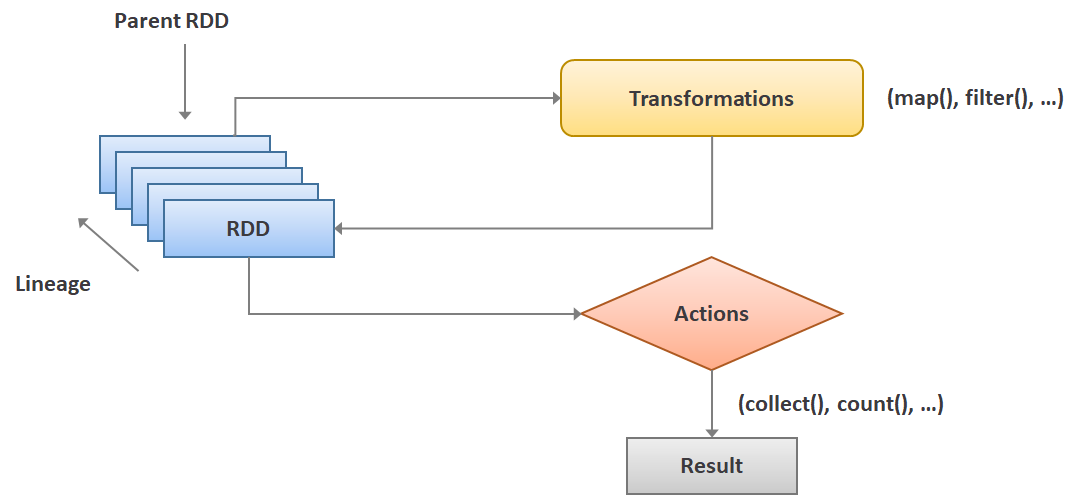
\includegraphics[height=5cm]{spark-rdd.png}
			\caption{Image 2 - RDD Operations}
		\end{figure}
	\end{center}
\end{frame}

\section{Spark Streaming}
\begin{frame}[t]{Spark Streaming}
	\begin{center}
		\begin{figure}
			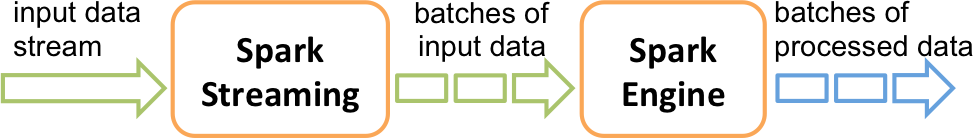
\includegraphics[height=1.5cm]{streaming-flow.png}
			\caption{Image 3 - Spark Streaming}
		\end{figure}
	\end{center}
	\begin{itemize}
		\item<2-> Mini batching - near-real time
		\item<3-> Legacy - there are better options now
		\item<4-> Abstract concept - \textbf{DStream} - Discretized Stream
		\begin{itemize}
			\item<5-> Continuous stream of data
			\item<6-> Represents a continuous sequence of RDDs
			\item<7-> Operations on DStream translates to operations on underlying RDDs
		\end{itemize}
	\end{itemize}
\only<7->{
	\begin{center}
		\begin{figure}
			\includegraphics<7->[height=1.2cm]{streaming-dstream.png}
			\caption{Image 4 - DStream RDDs}
		\end{figure}
	\end{center}
}
\only<8->{Therefore \mintinline{java}{DStream[T]} can be viewed as \mintinline{java}{RDD[RDD[T]]}}
\end{frame}

\begin{frame}{Spark Streaming}
	\begin{itemize}
		\item<1-> Input DStreams - representing the stream of input data
		\item<2-> Associted with \textbf{Receiver} - object which receives the data from a source, runs on an allocated core
		\begin{itemize}
			\item<3-> Reliable Receiver - sends ACK to the source
			\item<4-> Unrealiable Receiver - doesn't send ACK
			\item<5-> We can create custom receivers
		\end{itemize}
		\item<6-> Sources
		\begin{itemize}
			\item<7-> \textbf{Basic} - Available in \mintinline{java}{StreamingContext}: file systems and socket connections
			\item<8-> \textbf{Advanced} - Extra utility classes: Kafka, Flume, Kinesis
		\end{itemize}
		\item<9-> Drawbacks
		\begin{itemize}
			\item<10-> Directly dealing with RDDs
			\item<11-> Complicated and different API (from batch)
			\item<12-> Latency
			\item<13-> Bad Optimization
			\item<14-> SQL not supported
		\end{itemize}
	\end{itemize}
\end{frame}

\begin{frame}[t]{Spark Streaming}
\begin{itemize}
	\item<1-> DStream can be combined and joined
	\item<2-> For example, Window operations
\end{itemize}
\only<3->{
	\begin{center}
		\begin{figure}
			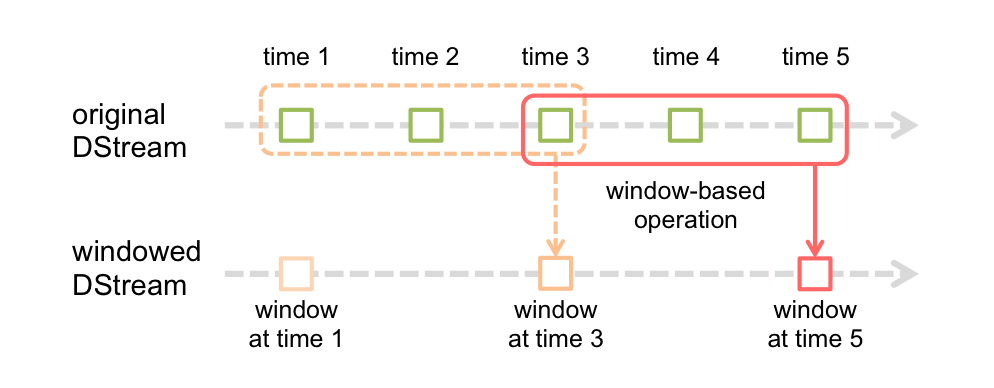
\includegraphics[height=4cm]{streaming-dstream-window.png}	
			\caption{Image 5 - DStream Window}
		\end{figure}
	\end{center}
}
\begin{center}
	\only<4->{However, DStream is not great for Stateful streams \\ and can't handle late data. There are other alternatives!}
\end{center}
\end{frame}

\section{DataFrame - DataSet}
\begin{frame}[t]{DataFrame/DataSet}
\begin{itemize}
	\item<1-> Introduced in Spark 2.0
	\item<2-> Built on top of RDDs
	\item<3-> Imposes a structure over data - columns/rows
	\item<4-> Dataset has two APIs - strongly-typed and untyped
	\item<5-> \mintinline{java}{Row} - generic untyped JVM object
\end{itemize}
\only<6>{
	\begin{center}
		\begin{figure}
			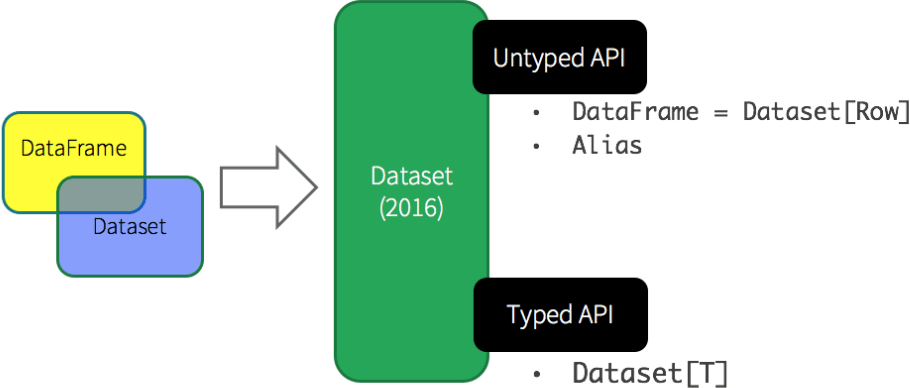
\includegraphics[height=3.5cm]{dataframe-dataset-api.png}
			\caption{Image 6 - DataFrame/DataSet}
		\end{figure}
	\end{center}
}
\only<7>{
\begin{center}
	\begin{tabular}{|c|l|}\hline
    	Language & Main Abstraction \\\hline
    	Scala & Dataset[T] \& DataFrame (alias for Dataset[Row]) \\\hline
    	Java & Dataset[T] \\\hline
    	Python & DataFrame \\\hline
    	R & DataFrame \\\hline
	\end{tabular}
\end{center}
}
\end{frame}

\begin{frame}[t]{DataFrame/DataSet}
Structure Benefits:
\begin{itemize}
	\item<1-> Syntax check, static-typing, runtime type-safety i.e. catch errors at compile time
	\item<2-> Simpler high-level operations - \mintinline{java}{agg}, \mintinline{java}{filter}, \mintinline{java}{groupBy}...
	\item<3-> Uses Spark SQL - has \href{https://www.databricks.com/glossary/catalyst-optimizer}{Catalyst Optimizer} which generates optimized logical and physical plan, together with \href{https://www.databricks.com/glossary/tungsten}{Tungstan}
\end{itemize}
\only<4>{
	\begin{center}
		\begin{figure}
			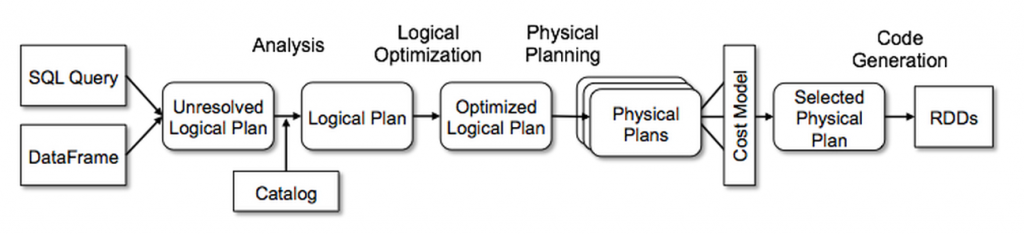
\includegraphics[height=2.5cm]{catalyst-optimizer.png}
			\caption{Image 7 - Catalyst Optimizer}
		\end{figure}
	\end{center}
}
\only<5>{
	\begin{center}
		\begin{figure}
			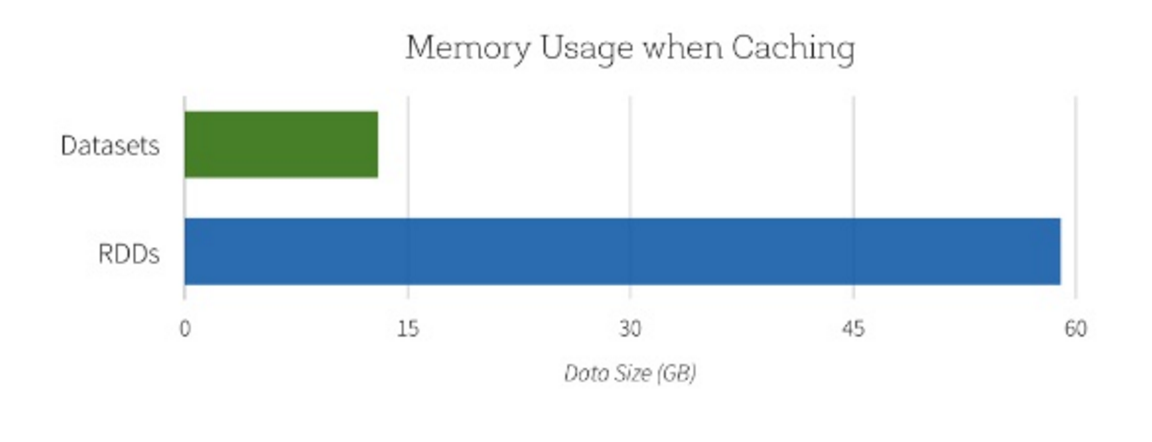
\includegraphics[height=3cm]{dataframe-space-efficiency.png}
			\caption{Image 8 - Memory Usage}
		\end{figure}
	\end{center}
}
\end{frame}

\section{Structured Streaming}
\begin{frame}{Structured Streaming}
Builds on top of structure provided by DataFrames/DataSets, which has its benefits:
\begin{itemize}
	\item<1-> Fast and scalable
	\item<2-> Fault-tolerant
	\item<3-> End-to-end exactly-once stream
	\item<4-> Stream and Batch are the same, we develop once
	\item<5-> Provides Event Time handling and Late Data processing - Watermarking
	\item<6-> Perform complex SQL queries
\end{itemize}
\end{frame}

\begin{frame}[t]{Structured Streaming}
How it works:
\only<1>{
	\begin{itemize}
		\item Unbounded Input Table
	\end{itemize}
}

\only<1>{
	\begin{center}
		\begin{figure}
			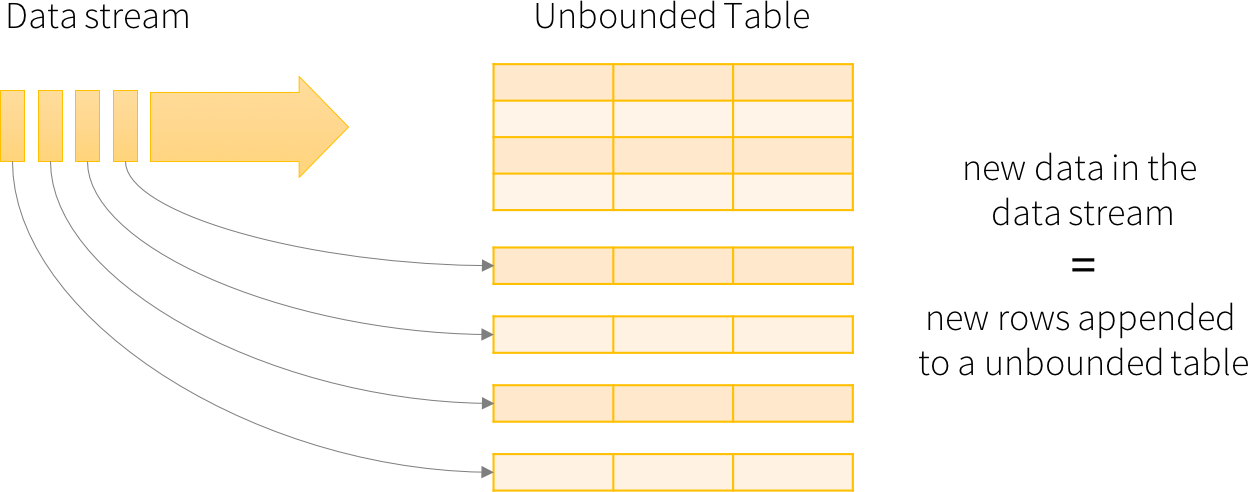
\includegraphics[height=4cm]{structured-streaming.png}
			\caption{Image 9 - Unbounded Table}
		\end{figure}
	\end{center}
}

\only<2>{
	\begin{itemize}
		\item Result Table
	\end{itemize}
}

\only<2>{
	\begin{center}
		\begin{figure}
			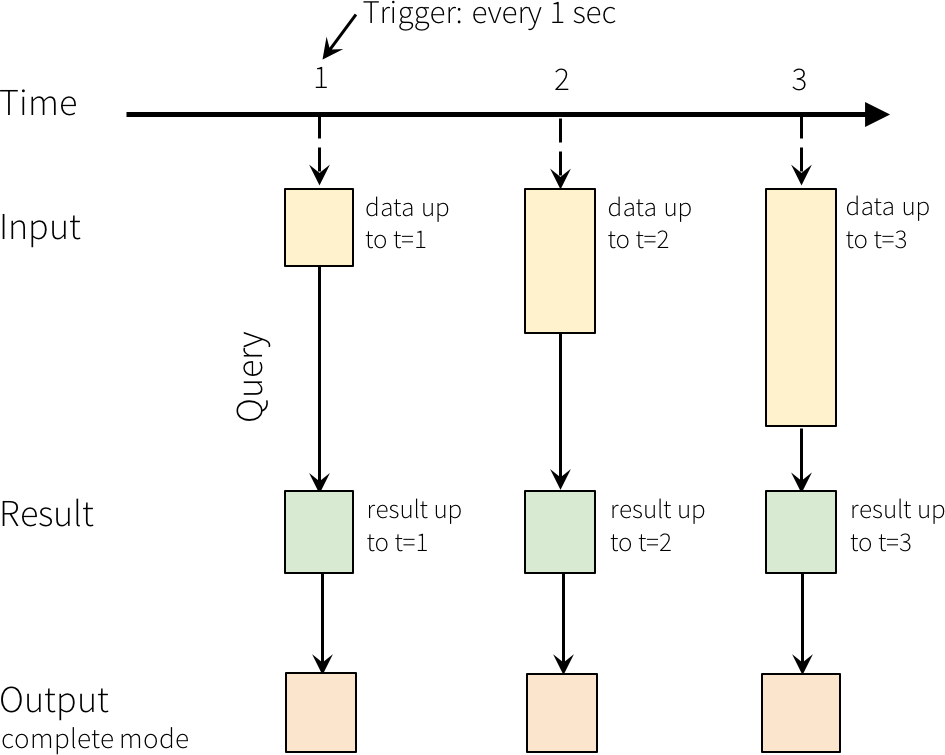
\includegraphics[height=5cm]{structured-streaming-model.png}
			\caption{Image 10 - Result Table}
		\end{figure}
	\end{center}
}
\end{frame}

\begin{frame}[t]{Structured Streaming}
\begin{itemize}
	\item<1-> Output Modes - defines what gets written to the external storage
	\begin{itemize}
		\item<2-> \textbf{Complete} - Complete result tables are written
		\item<3-> \textbf{Append} - Only rows that get appended since the last trigger
		\item<4-> \textbf{Update} - Only rows that were updated
	\end{itemize}
\end{itemize}
\only<5->{
	\begin{center}
		\begin{figure}
			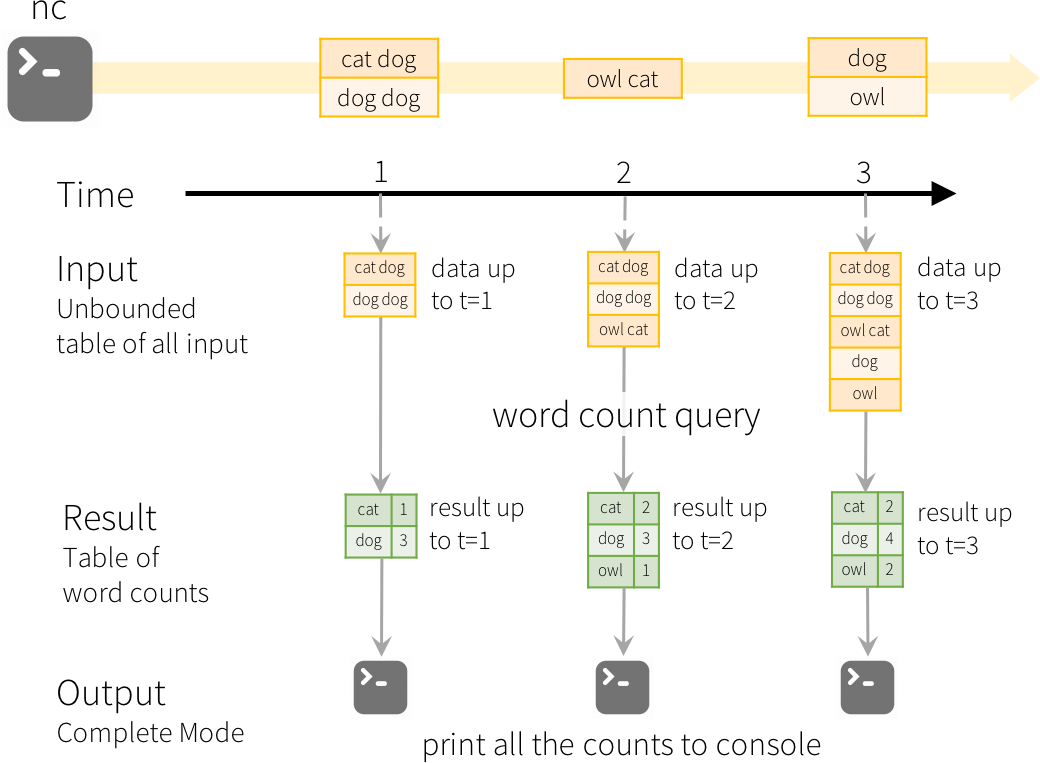
\includegraphics[height=5cm]{structured-streaming-example-model.png}
			\caption{Image 11 - Query Example}
		\end{figure}
	\end{center}
}
\end{frame}

\begin{frame}{Structured Streaming}
Window operations
\only<1>{
	\begin{center}
		\begin{figure}
			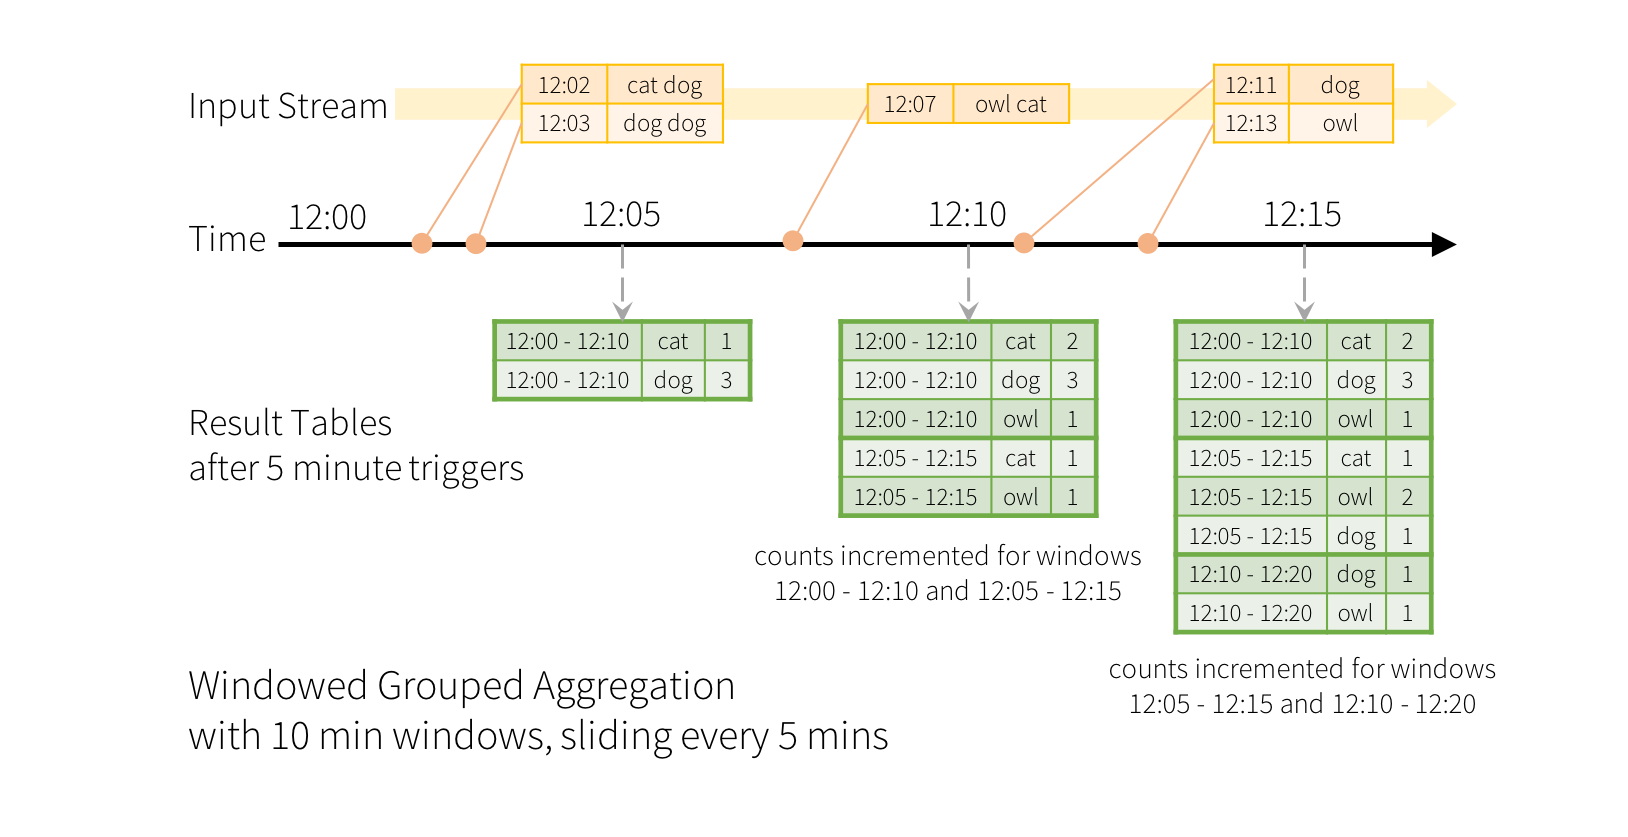
\includegraphics[height=6cm]{structured-streaming-window.png}
			\caption{Image 12 - Window Operation}
		\end{figure}
	\end{center}
}
\end{frame}

\begin{frame}[fragile]{Watermarking}
\begin{itemize}
	\item<1-> Introduced in Spark 2.1
	\item<2-> Keeps track of event time in data
	\item<3-> Engine maintains state and allow late data for specific window \mintinline{java}{T}
	\item<4-> Regulates state - cleaning\\
	\item<5-> {Example:
	\scriptsize
\begin{minted}{python}

	words = ...  # streaming DataFrame

	# Group the data by window
	windowedCounts = words \
    	.withWatermark("timestamp", "10 minutes") \
    	.groupBy(
        	window(words.timestamp, "10 minutes", "5 minutes"),
        	words.word) \
    	.count()
\end{minted}
}
\end{itemize}

\end{frame}

\begin{frame}{Watermark}
\only<1>{
	\begin{center}
		\begin{figure}
			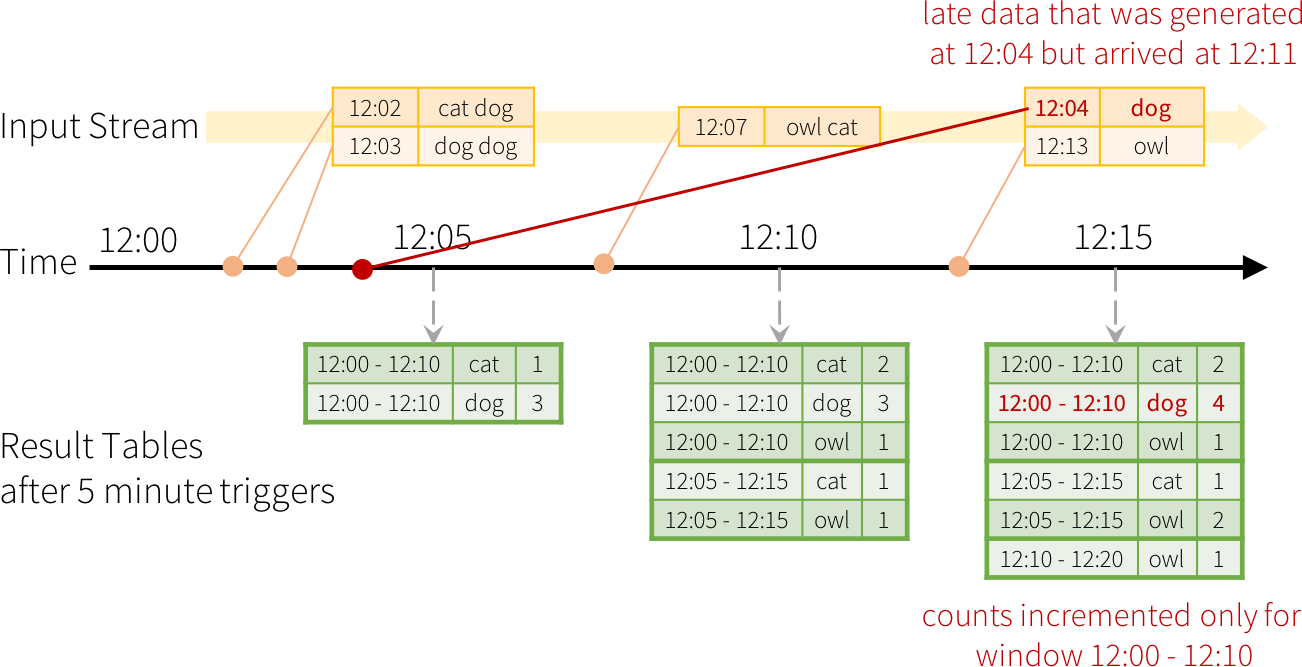
\includegraphics[height=5cm]{structured-streaming-late-data.png}
			\caption{Image 13 - Watermark}
		\end{figure}
	\end{center}
}
\end{frame}

\begin{frame}
\begin{center}
\huge{THANKS!}\\[2ex]
\normalsize{If you have any questions, please don't hesitate to ask}
\end{center}
\end{frame}

\section*{References}
\begin{frame}{References}
	\begin{itemize}
		\item{Spark Official Documentation}
		\begin{itemize}
			\item{\href{https://spark.apache.org/docs/latest/rdd-programming-guide.html}{RDD Programming Guide}}
			\item{\href{https://spark.apache.org/docs/latest/streaming-programming-guide.html}{Streaming Programming Guide}}
			\item{\href{https://spark.apache.org/docs/latest/structured-streaming-programming-guide.html}{Structured Streaming Programming Guide}}
		\end{itemize}
		\item{Databricks}
		\begin{itemize}
			\item{\href{https://www.databricks.com/blog/2016/07/14/a-tale-of-three-apache-spark-apis-rdds-dataframes-and-datasets.html}{A Tale of Three Apache Spark APIs: RDDs vs DataFrames and Datasets}}
			\item{\href{https://www.databricks.com/blog/multiple-stateful-operators-structured-streaming}{Multiple Stateful Operators in Structured Streaming}}
		\end{itemize}
		
	\end{itemize}
\end{frame}

\section*{Images}
\begin{frame}
Images
\begin{itemize}
	\item Image 1 - Partitions - \href{https://towardsdata.dev/apache-spark/2022/spark-bucketing-and-partitions}{Source}
	\item Image 2 - RDD Operations - \href{https://medium.com/analytics-vidhya/spark-rdd-low-level-api-basics-using-pyspark-a9a322b58f6}{Source}
	\item Image 3 - Spark Streaming - \href{https://spark.apache.org/docs/latest/streaming-programming-guide.html}{Source}
	\item Image 4 - DStream RDDs - \href{https://spark.apache.org/docs/latest/streaming-programming-guide.html}{Source}
	\item Image 5 - DStream Window - \href{https://spark.apache.org/docs/latest/streaming-programming-guide.html}{Source}
	\item Image 6 - DataFrame/DataSet - \href{https://www.databricks.com/blog/2016/07/14/a-tale-of-three-apache-spark-apis-rdds-dataframes-and-datasets.html}{Source}
	\item Image 7 - Catalyst Optimizer - \href{https://www.databricks.com/glossary/catalyst-optimizer}{Source}
	\item Image 8 - Memory Usage - \href{https://www.databricks.com/blog/2016/07/14/a-tale-of-three-apache-spark-apis-rdds-dataframes-and-datasets.html}{Source}
	\item Image 9 - Unbounded Table - \href{https://spark.apache.org/docs/latest/structured-streaming-programming-guide.html}{Source}
	\item Image 10 - Result Table - \href{https://spark.apache.org/docs/latest/structured-streaming-programming-guide.html}{Source}
	\item Image 11 - Query Example - \href{https://spark.apache.org/docs/latest/structured-streaming-programming-guide.html}{Source}
	\item Image 12 - Window Operation - \href{https://spark.apache.org/docs/latest/structured-streaming-programming-guide.html}{Source}
	\item Image 13 - Watermark - \href{https://spark.apache.org/docs/latest/structured-streaming-programming-guide.html}{Source}
\end{itemize}
\end{frame}

\end{document}
